\documentclass[a4paper,14pt]{extarticle}
%\makeatletter
%\makeatother
\usepackage[margin=1in]{geometry}
\usepackage{subcaption}
\usepackage{multirow}
\usepackage{graphicx}
%%
%%\usepackage{color}
%%\usepackage{minted}
%%\usepackage[russian]{hyperref}
%%
\graphicspath{{./pictures/}}
\DeclareGraphicsExtensions{.pdf,.png,.jpg}
\usepackage{amsmath,amsthm,amssymb}
\usepackage{mathtext}
\usepackage[T1,T2A]{fontenc}
\usepackage[utf8]{inputenc}
\usepackage[english, russian]{babel} % указать, что язык текста - русский
\usepackage{amsmath, amsfonts, amssymb, amsthm,mathtools}
\usepackage[shortcuts,cyremdash]{extdash}
%\usepackage{fancyhdr}
%\pagestyle{fancy}
\usepackage{wrapfig}
\usepackage{romannum}
\begin{document}

\begin{titlepage}
\begin{center}


\textsc{\Large Лабораторная работа 5.1.3: \\ }

% Title
\HRule \\[0.4cm]
{ \LARGE \bfseries Эффект Рамзауэра. }

\HRule \\[1.5cm]

% Author and supervisor
\noindent
\begin{minipage}{0.4\textwidth}
\begin{flushleft} \large
\end{flushleft}
\end{minipage}%
\begin{minipage}{0.4\textwidth}
\begin{flushright} \large
\end{flushright}
\end{minipage}

\large{\begin{flushright}
\vfill
\textbf{Выполнила}:\\
\textbf{Шигаева Маргарита\\}
\textbf{группа Б05-871}
\end{flushright}}

{\large \today}\\

\end{center}
\end{titlepage}




\section{Цель} % (fold)
\label{sec:цель}
Исследовать энергетическую зависимость вероятности рассеяния жлектронов атомами ксенона, определяются энергии электронов, при которых наблюдается `Просветление` ксенона, и оценивается размер его внешней электронной оболочки.
% section цель (end)

\section{Схема установки} % (fold)
\label{sec:схема_установки}

\begin{figure}[h!]
	\centering
	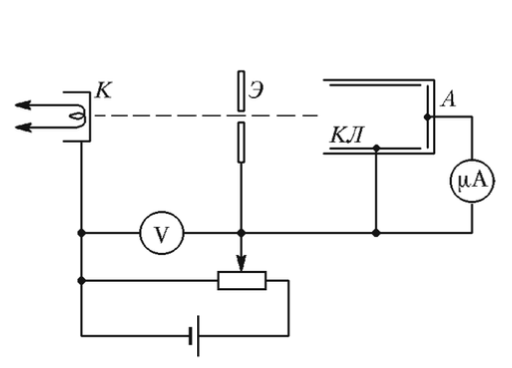
\includegraphics[width = 0.7\linewidth]{scheme_513}
	\caption{Схема установки для измерения сечения рассеяныхэлектронов в газах}	
\end{figure}
Пучок электронов вылетает из накаленного катода К, проходит ускоряющую разность потенциалов V, приложенную между катодом и электродом Э, и приобретает энергию $E = \frac{mv^2}{2} = eV$. ПРи прохождении через газ часть электронов рассеивается на атомах, уходит в сторону и собирается коллектором КЛ, а прощедшие без рассеяния электроны попадают на анод А и создают анодный ток I. 
% section схема_установки (end)

\section{Теоритическая часть} % (fold)
\label{sec:Теоритическая_часть}
	Рассмотрим атомы газа как сферическую потенциальную яму. Это сложно, поэтому рассмотрим более грубую модель, одномерную потенциальную яму прямоугольной формы, эта модель хорошо отличается для атомов тяжелых инертных газов, отличащихся компактной структурой и резкой внешней границей. Решение задачи о прошохдении частицы с энергией E над потенциальной ямой шириной l и глубиной $U_0$ 
	\begin{wrapfigure}{l}{0.4\linewidth}
	\centering
	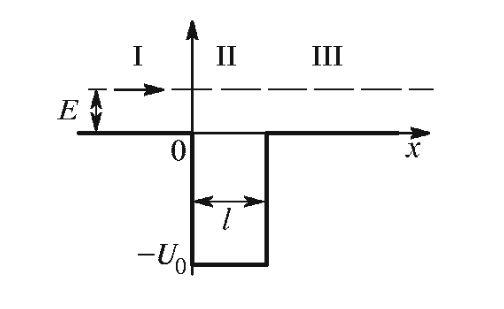
\includegraphics[width = \linewidth]{potential_pit}
	\caption{Задача об одномерной потенциальной яме}
	\end{wrapfigure}
	Уравнение Шредингера в областях \Romannum{1}, \Romannum{2}, \Romannum{3} имеет вид: 
	\begin{equation*}
		\psi'' + k^2\psi = 0 \text{, где } k^2 = \begin{cases}
			k_1^2 = \frac{2mE}{\hbar^2}& \text{\Romannum{1} и \Romannum{3}}  \\
			k_2^2 = \frac{2m(E+U_0)}{\hbar^2}& \text{\Romannum{2} }  
		\end{cases}
	\end{equation*}
	Найдем коэффициент прохождения через барьер:
	\begin{equation*}
	  	D = \frac{j_{прош}}{j_{пад}} = \frac{16k_1^2k_2^2}{16k_1^2k_2^2+ 4(k_1^2-k_2^2)^2sin^2(k_2l)}
	\end{equation*}  
	Видно, что коэффициент прохождения частицы над ямой имеет чередующиеся минимумы и максимумы в зависимости от энергии. Если $k_2l = \pi + 2\pi n$, то коэффициент прохождения равен 1, то есть электрон беспрепятственно проходит через атом.
	Таким образом условие максимального коэффициента пропускания:
	\begin{equation}
		k_2l = \sqrt{\frac{2m(E+U_0)}{\hbar^2}l} = \pi n
	\end{equation}
	Условие первого дифференционного максимума
	\begin{equation}
		2l = \frac{h}{\sqrt{2m(E_1+U_0}}
	\end{equation}
	Условие первого интереференционного минимума
	\begin{equation}
		2l = \frac{3}{2}\frac{h}{\sqrt{2m(E_2+U_0)}}
	\end{equation}
	\begin{equation}
		l = \frac{h\sqrt{5}}{\sqrt{32m(E_2-E_1)}}
	\end{equation}
	Эффективная глубина потенциальной ямы:
	\begin{equation}
		U_0 = \frac{4}{5}E_2-\frac{9}{5}E_1.
	\end{equation}
	% section вывод (end)

	\section{Ход работы} % (fold)
	\label{sec:ход_работы}
	\subsection{Динамический режим} % (fold)
	\label{sub:динамический_режим}
	
	% subsection динамический_режим (end)
	Измерим напряжения на катоде для максимумы и минимумов на аноде в динамическом режиме
	\begin{table}[h!]
		\centering
		\caption{Экстремумы в ВАХ}
		\begin{tabular}{|c|c|c|}
		\hline
			напряжение накала, В&$V_1\text{(максимум), В}$&$V_2\text{(минимум), В}$\\ \hline
			3 & 2,34&7,1 \\ \hline
			2,6 & 2,31 &7,42 \\ \hline
		\end{tabular}
	\end{table}
	По формулам (2)-(5) определим размер электронной оболочки
	получим 
	$l_{\textnormal{ср}} = 2,94\cdot 10^{-10}м$ и относительня погрешность $\varepsilon = 2,21\% \implies$
	$$
		l\approx(2,94\pm0,07)\cdot 10^{-10}\text{м}
	$$
	По формуле(5) оценим глубину потенциальной ямы $U_0$
	\begin{table}[h!]
		\centering
		\begin{tabular}{|c|c|}
		\hline
			Напряжение накала,B & $U_0,B$\\ \hline
			3 & 2,89 \\ \hline
			2,6 & 3,26\\ \hline
		\end{tabular}
	\end{table}
	По результатам измерения напряжения пробоя оценим потенциал ионизации инертного газа.
	$$
	I = 12,5\pm0,5 \implies \text{титатрон наполнен ксеноном} 
	$$
	\subsection{Статистический режим} % (fold)
	\label{sub:статистический_режим}
	
	% subsection статистический_режим (end)
	Теперь применим статистический метод.

	Снимем зависимость тока на аноде от напряжения.
	\begin{table}[h!]
		\centering
		\caption{Зависимость тока на аноде от напряжения при напряжении накала 3,0В}
		\begin{tabular}{|c|c|} 
		\hline
		Напряжение катода, В&Напряжение Анода, В  \\ \hline
			0,07	&	-0,02	\\ \hline
0,5	&	-0,02	\\ \hline
0,74	&	-0,02	\\ \hline
1,03	&	0	\\ \hline
1,2	&	0,04	\\ \hline
1,25	&	0,07	\\ \hline
1,295	&	0,12	\\ \hline
1,33	&	0,2	\\ \hline
1,37	&	0,29	\\ \hline
1,395	&	0,38	\\ \hline
1,408	&	0,44	\\ \hline
1,42	&	0,52	\\ \hline
1,45	&	0,66	\\ \hline
1,47	&	0,87	\\ \hline
1,49	&	1	\\ \hline
1,51	&	1,14	\\ \hline
1,54	&	1,61	\\ \hline
1,58	&	2,25	\\ \hline
1,59	&	2,77	\\ \hline
1,605	&	3,16	\\ \hline
1,61	&	3,45	\\ \hline
1,62	&	3,86	\\ \hline
1,635	&	4,38	\\ \hline
1,65	&	5,08	\\ \hline
1,66	&	5,8	\\ \hline
1,69	&	7,5	\\ \hline
1,675	&	6,52	\\ \hline
1,707	&	8,67	\\ \hline
1,718	&	9,5	\\ \hline
1,73	&	10,3	\\ \hline
1,75	&	12,6	\\ \hline
1,761	&	13,5	\\ \hline
1,77	&	14,9	\\ \hline
1,786	&	16,5	\\ \hline
1,796	&	18,2	\\ \hline
1,8	&	18,6	\\ \hline
1,81	&	20	\\ \hline
		\end{tabular}
		\begin{tabular}{|c|c|} 
			\hline
			1,824	&	22,03	\\ \hline
1,83	&	22,9	\\ \hline
1,85	&	26,4	\\ \hline
1,87	&	29,7	\\ \hline
1,89	&	34,3	\\ \hline
1,91	&	36,9	\\ \hline
1,93	&	41,9	\\ \hline
1,94	&	43,9	\\ \hline
1,974	&	50,3	\\ \hline
2	&	55,4	\\ \hline
2,026	&	60,5	\\ \hline
2,077	&	69,5	\\ \hline
2,114	&	75,5	\\ \hline
2,2	&	86,8	\\ \hline
2,28	&	90,4	\\ \hline
2,3	&	91,14	\\ \hline
2,34	&	91,87	\\ \hline
2,42	&	91,38	\\ \hline
2,48	&	90,37	\\ \hline
2,51	&	89,8	\\ \hline
2,55	&	88,2	\\ \hline
2,63	&	84,6	\\ \hline
2,71	&	81,4	\\ \hline
2,806	&	77,3	\\ \hline
2,96	&	72,2	\\ \hline
3,1	&	69,2	\\ \hline
3,34	&	63,6	\\ \hline
3,7	&	58,4	\\ \hline
4,27	&	53,5	\\ \hline
4,88	&	49,1	\\ \hline
5,56	&	45,65	\\ \hline
7,1	&	42,36	\\ \hline
7,5	&	42,6	\\ \hline
7,36	&	42,54	\\ \hline
8,27	&	43,9	\\ \hline
9,1	&	48,1	\\ \hline
10,4	&	56,75	\\ \hline
10,88	&	65	\\ \hline
		\end{tabular}
	\end{table}
	\begin{table}[h!]
	\centering
	\caption{Зависимость тока на аноде от напряжения при напряжении накала 2,6 В}
	\begin{tabular}{|c|c|}
		\hline
		Напряжение катода, В&Напряжение Анода, В  \\ \hline
		0,01	&	0,02	\\ \hline
0,16	&	0,02	\\ \hline
0,25	&	0,01	\\ \hline
0,32	&	0,01	\\ \hline
0,42	&	0,01	\\ \hline
0,55	&	0,01	\\ \hline
0,85	&	0,01	\\ \hline
1,09	&	0	\\ \hline
1,171	&	0,01	\\ \hline
1,25	&	0,02	\\ \hline
1,35	&	0,03	\\ \hline
1,37	&	0,06	\\ \hline
1,57	&	0,46	\\ \hline
1,62	&	0,66	\\ \hline
1,68	&	1,28	\\ \hline
1,73	&	2,17	\\ \hline
1,8	&	4,5	\\ \hline
1,93	&	11,07	\\ \hline
2	&	15,3	\\ \hline
2,15	&	20,1	\\ \hline
2,27	&	22,53	\\ \hline
2,31	&	22,68	\\ \hline
2,32	&	22,67	\\ \hline
2,33	&	22,63	\\ \hline
2,39	&	22,22	\\ \hline
2,41	&	21,9	\\ \hline
2,45	&	21,73	\\ \hline
2,54	&	20,5	\\ \hline
2,7	&	18,53	\\ \hline
2,79	&	17,66	\\ \hline
2,9	&	16,66	\\ \hline
3	&	15,67	\\ \hline
3,47	&	13,71	\\ \hline
3,8	&	12,8	\\ \hline
4	&	12,35	\\ \hline
4,2	&	12,1	\\ \hline
4,32	&	11,87	\\ \hline
	\end{tabular}
	\begin{tabular}{|c|c|}
		\hline
		V&V \\ \hline
		4,4	&	11,7	\\ \hline
4,53	&	11,5	\\ \hline
4,7	&	11,3	\\ \hline
5	&	10,9	\\ \hline
5,2	&	10,6	\\ \hline
5,43	&	10,4	\\ \hline
5,556	&	10,3	\\ \hline
5,7	&	10,2	\\ \hline
5,88	&	10,1	\\ \hline
6	&	10,02	\\ \hline
6,83	&	9,8	\\ \hline
6,85	&	9,78	\\ \hline
6,86	&	9,79	\\ \hline
6,88	&	9,79	\\ \hline
6,92	&	9,82	\\ \hline
6,94	&	9,83	\\ \hline
7,1	&	9,8	\\ \hline
7,2	&	9,74	\\ \hline
7,264	&	9,7	\\ \hline
7,37	&	9,69	\\ \hline
7,398	&	9,68	\\ \hline
7,42	&	9,63	\\ \hline
7,45	&	9,65	\\ \hline
7,52	&	9,65	\\ \hline
7,6	&	9,65	\\ \hline
7,69	&	9,67	\\ \hline
7,78	&	9,67	\\ \hline
7,93	&	9,76	\\ \hline
8	&	9,8	\\ \hline
8,24	&	9,92	\\ \hline
8,85	&	10,45	\\ \hline
9,1	&	10,7	\\ \hline
9,87	&	11	\\ \hline
9,97	&	11,1	\\ \hline
10,25	&	11,86	\\ \hline
10,9	&	14,42	\\ \hline
11,4	&	14,8	\\ \hline
	\end{tabular}
	\end{table}
	\clearpage
	По этим данным построим графики зависимости
	\begin{figure}[h!]
		\centering
		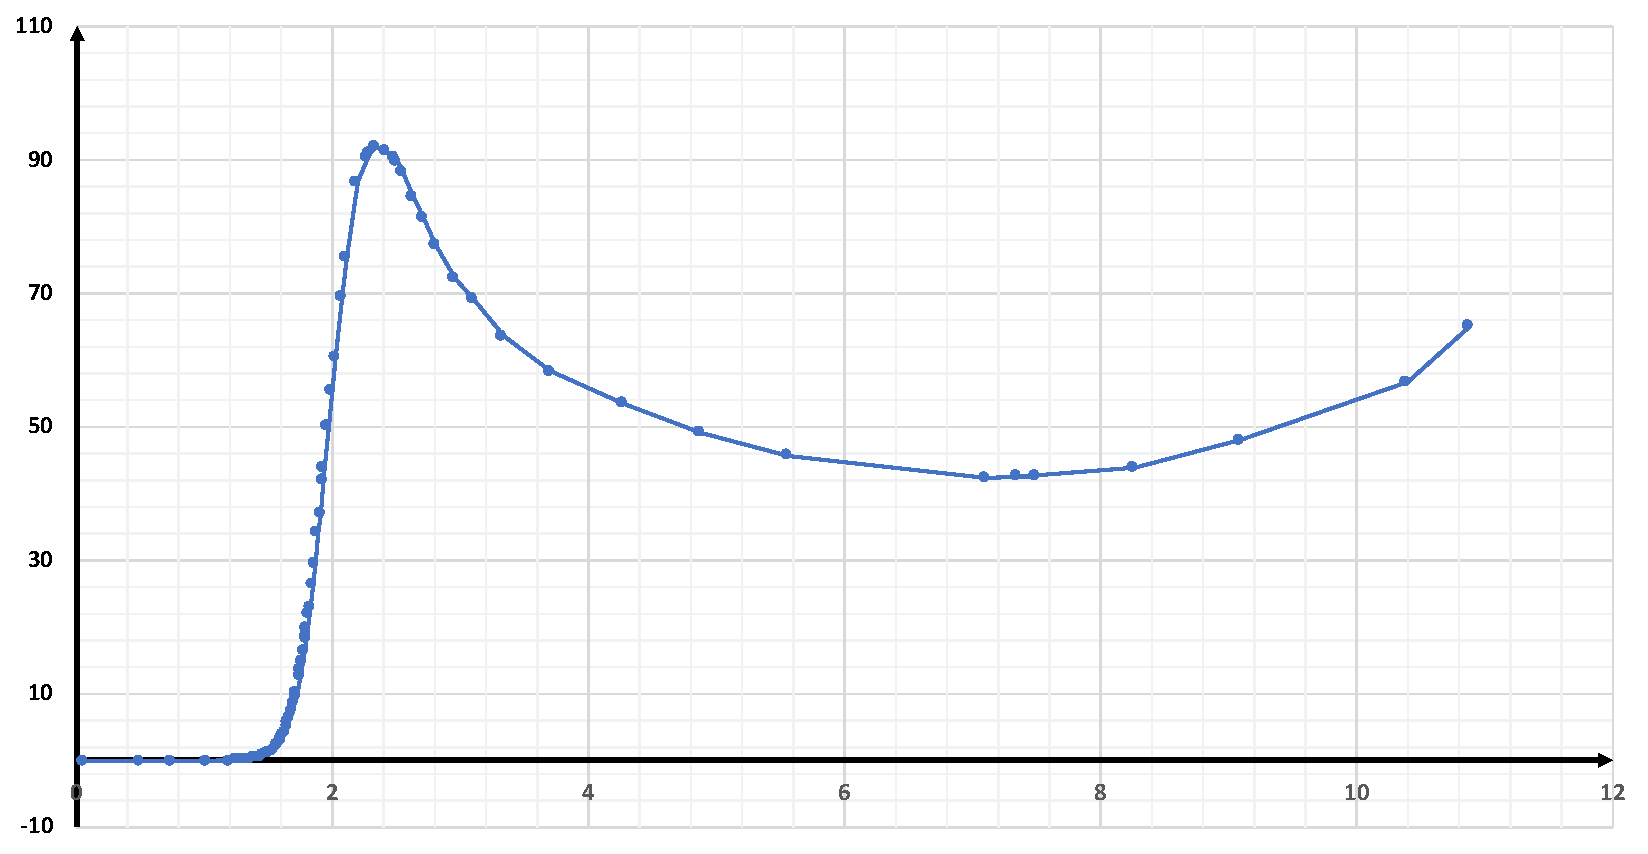
\includegraphics[width = \linewidth]{I(V)_1}
		\caption{График зависимости $I_a(V)$ при напряжении накала 3,0 В}
	\end{figure}
	\begin{figure}[h!]
		\centering
		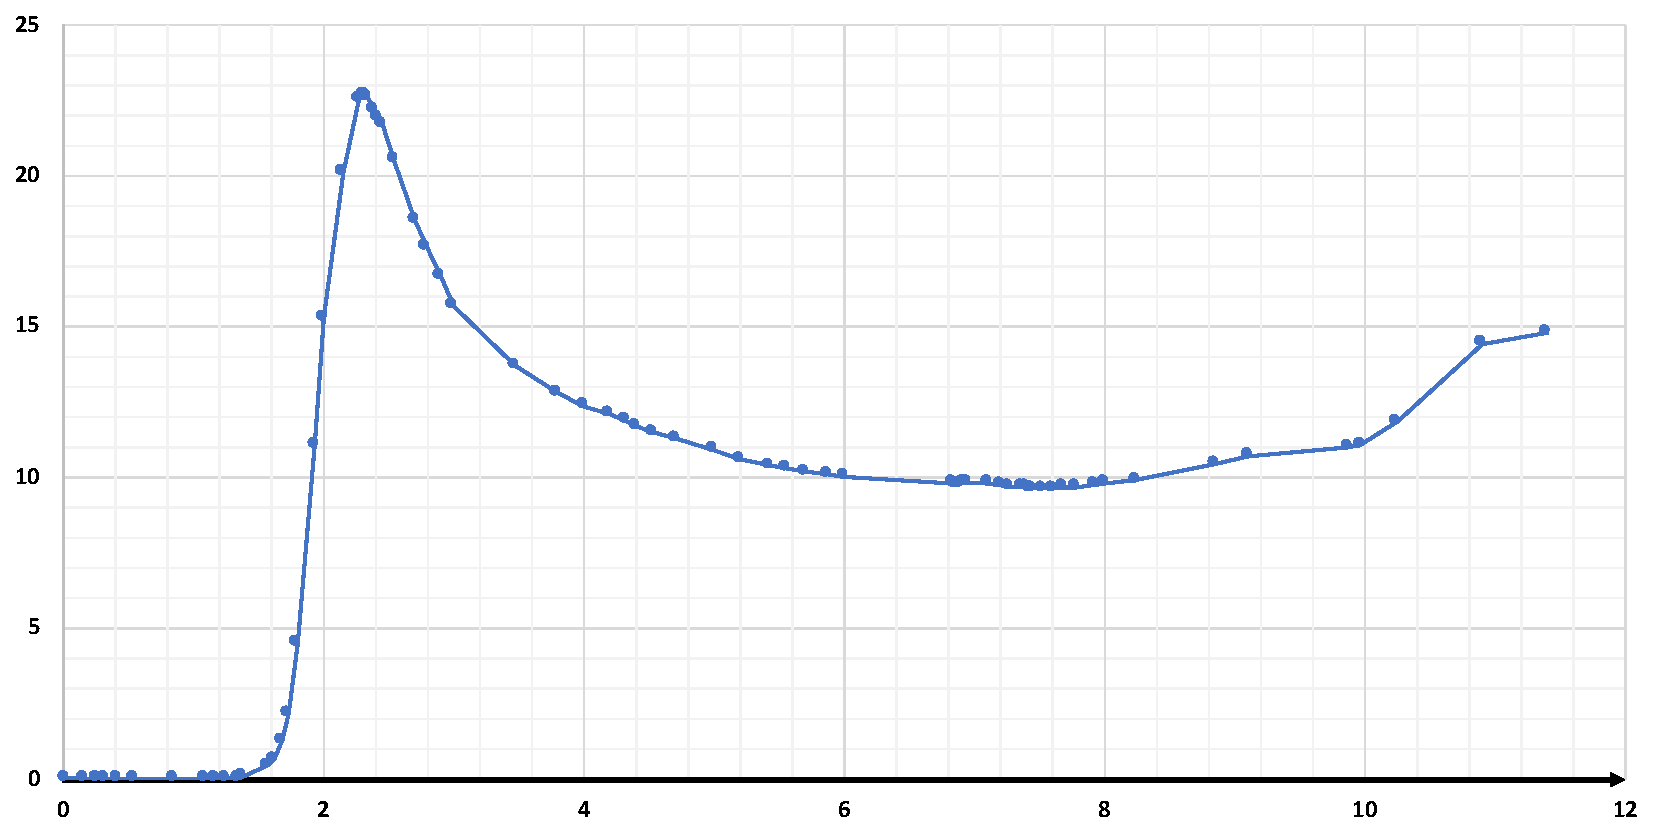
\includegraphics[width = \linewidth]{I(V)_2}
		\caption{График зависимости $I_a(V)$ при напряжении накала 2,6 В}
	\end{figure}
	Вычислим значения $l,U_0$
	\begin{table}[h!]
		\centering
		\caption{l,$U_0$ в статистическом методе}
		\begin{tabular}{|c|c|c|}
		\hline
			Напряжение накала, B & l, $10^{-10}$м& $U_0$,В \\ \hline
			3 & 2,97& 2,89 \\ \hline
			2,6& 2,86& 3,26 \\ \hline
		\end{tabular}
	\end{table}
	%\clearpage
	Оценим напряжения про которых должны появляться максимумы в коэффициенте прохожденияя электронов для n = 2,3 по формуле (1):
	$$
		k_2l = \sqrt{\frac{2m(E_n-E_0}{\hbar^2}} = \pi n
	$$
	$\implies$
	$$
		E_n = \frac{(\pi n \hbar)^2}{2ml^2}-U_0, \ где	
	$$
	$
		\hbar = 1,05\cdot10^{-34} \ Дж\cdotс\\
		U_0 = 2,5 \ эВ\\
		m = 9,11\cdot10^{-31} \ кг\\
		l = 3,0\cdot10^{-10} \ м\ (с \ учетом \ вычисления\  для U_{нак} = 2,6 \ В \ и \ U_{нак} = 3,0 \ В)\implies
	$
	$$
	E_2 \approx 20,9 \ эВ, \ U_2 \approx 20,9 \ В\\
	$$
	$$
	E_3 \approx 52,0 \ эВ, \ U_3 \approx 52,0 \ В\\
	$$
	По формуле $ \omega(U) = -\frac{1}{c}\ln(\frac{U_а(U)}{U_0})$ определим вероятность рассеивания электронов (с точностью до константы), где $U_0 = U_{нак}$

	\begin{figure}[h!]
		\centering
		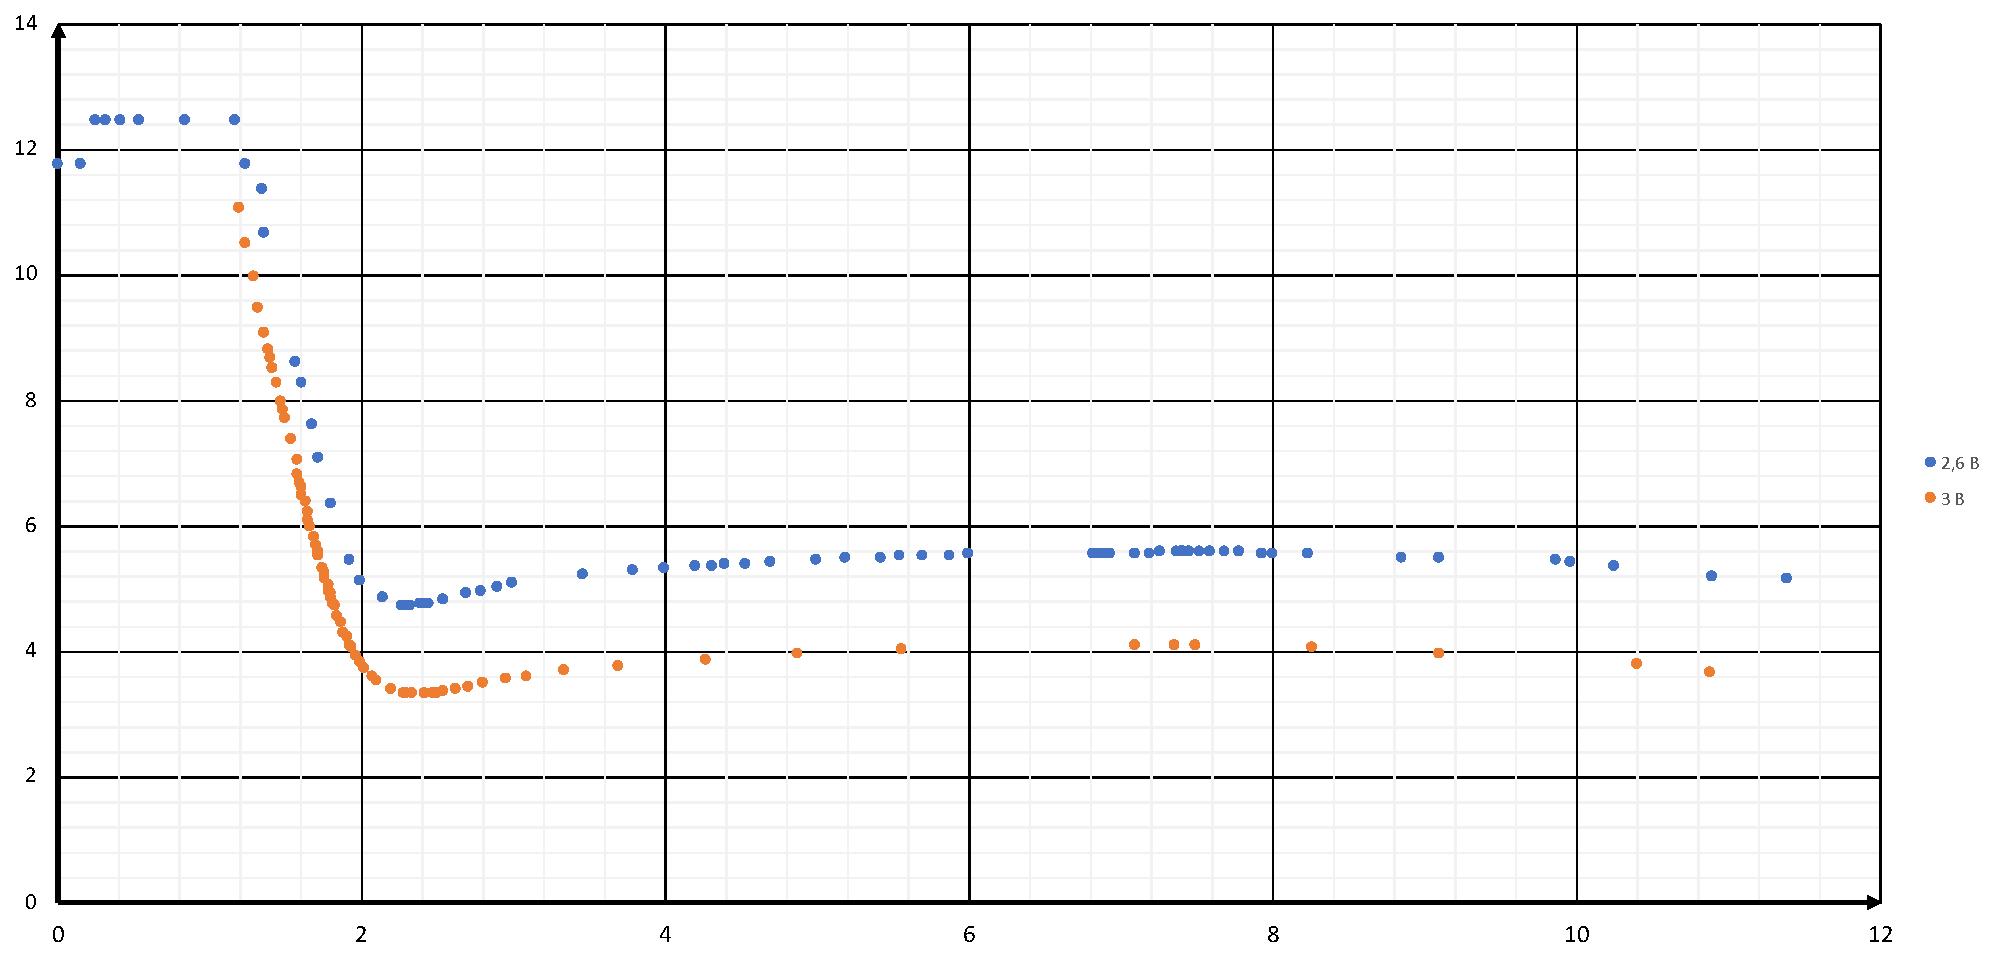
\includegraphics[width = \paperwidth]{graph_2_513}
		\caption{Зависимость вероятности рассеивания электронов от напряжения на катоде}
	\end{figure}
	% section ход_работы (end)
	\clearpage
	\section{Итоговые результаты} % (fold)
	\label{sec:итоговые_результаты}
	\begin{table}[h!]
		\centering
		\caption{итоговая таблица}
		\begin{tabular}{|c|c|c|c|c|}
			\hline
			Напряжение накала & U_0, В& l, $10^{-10}м$&$U_1, В$ & $U_2, В$ \\ \hline
			Для $U_{нак}=2,6$ В& 3,26& 2,86& 2,31&7,42\\ \hline
			Для $U_{нак}=3,0$ В& 2,89& 2,97& 2,34&7,1 \\ \hline
		\end{tabular}
		
	\end{table}
	% section итоговые_результаты (end)

	\section{Вывод} % (fold)
	\label{sec:вывод}
	В процессе работы исследовались энергетическую зависимость вероятности рассеивания электронова атомами инертного газа, определили электроны, при которых наблюдается просветлене и оценили размер внешней оболочки атома.
	% section вывод (end)
\end{document}
